\chapter{Funções especiais e equações com coeficientes variáveis}
Nesse capítulo discutiremos a transformada de Laplace envolvendo funções especiais, tais como função de Bessel, função Gama e funções Seno Integrado. Também, desenvolveremos ferramentas capaz de resolver alguns problemas de valor iniciais com coeficientes não constantes.
Para iniciar as discussões vamos demonstrar o item 6 da tabela \ref{tab_trans_Lap_1} no próximo exemplo.
\begin{ex}Vamos calcular a transformada de Laplace da funçao $t^{k-1}$, dada por:
$$
\mathcal{L}\{t^{k-1} \}=\int_0^\infty t^{k-1} e^{-st}dt.
$$
Fazemos a mudança de variável $x=st$ para obter:
\begin{eqnarray*}
 \mathcal{L}\{t^{k-1} \}&=&\int_0^\infty \frac{x^{k-1}}{s^{k-1}}e^{-x}\frac{dx}{s}\\
 &=&\frac{1}{s^k}\int_0^\infty x^{k-1}e^{-x} dx.
 \end{eqnarray*}
A função que aparece acima é a multiplicação de $\frac{1}{s^k}$ por uma que não depende de $s$, chamada de função Gama e denotada por $\Gamma(k)$. Portanto, demonstramos o item (6) da tabela \ref{tab_trans_Lap_1}:
$$
\mathcal{L}\{t^{k-1} \}=\frac{\Gamma(k)}{s^k},\qquad k>0,
$$
onde
$$
\Gamma(k)=\int_0^\infty e^{-x}x^{k-1}dx.
$$
\end{ex}
Observe que o item 3 da tabela é
$$
\mathcal{L}\{t^{n-1}\}=\frac{(n-1)!}{s^n}, \qquad n\in \mathbb{N}.
$$
Isso nos indica que, para que os itens 3 e 6 sejam consistentes, $\Gamma(n+1)=n!$ se $n\in\mathbb{N}$. De fato, primeiro observe que, se $k=(n+1)\in\mathbb{N}$, temos:
$$
\Gamma(n+1)=\int_0^\infty e^{-x}x^{n}dx=\left[-e^{-x}x^{n}\right]_0^\infty-\int_0^\infty (-e^{-x})nx^{n-1}dx=n\int_0^\infty e^{-x}x^{n-1}dx=n\Gamma(n).
$$
Como 
$$
\Gamma(1)=\int_0^\infty e^{-x}dx=\left[-e^{-x}\right]_0^\infty=1,
$$
temos
$$
\Gamma(2)=1,\qquad \Gamma(3)=2\cdot 1=2!,\qquad \Gamma(4)=3\Gamma(3)=3\cdot 2!=3!,\cdots
$$
Logo, $\Gamma(n+1)=n!$ se $n\in\mathbb{N}$.
\begin{ex} Os itens 4 e 5 da tabela são casos particulares do item 6:
 $$
 \mathcal{L}\{t^{-\frac{1}{2}}\}=\frac{\Gamma\left(\frac{1}{2}\right)}{s^{\frac{1}{2}}}
 $$
e
 $$
 \mathcal{L}\{t^{\frac{1}{2}}\}=\frac{\Gamma\left(\frac{3}{2}\right)}{s^{\frac{3}{2}}}.
 $$
 Basta calcular os valores de $\Gamma\left(\frac{1}{2}\right)$ e $\Gamma\left(\frac{3}{2}\right)$ para completar a demonstração. Começamos com $\Gamma\left(\frac{1}{2}\right)$:
 $$
 \Gamma\left(\frac{1}{2}\right)=\int_0^\infty e^{-x}x^{-\frac{1}{2}}dx=\int_0^\infty \frac{e^{-x}}{\sqrt{x}}dx.
 $$
 Fazendo a mudança de variáveis $x=t^{2}$, obtemos $dx=2tdt$ e
$$\Gamma\left(\frac{1}{2}\right)=2\int_{0}^{\infty}e^{-t^2}dt
$$
Utilizando a técnica de Liouville, definimos:
$$
I=\int_{0}^{\infty}e^{-t^2}dt
$$
Logo
$$
I^2=\int_{0}^{\infty}e^{-x^2}dx\int_{0}^{\infty}e^{-y^2}dy=\int_{0}^{\infty}\int_{0}^{\infty}e^{-(x^2+y^2)}dx dy
$$
A última integral é uma integral dupla que pode ser calculada em coordenadas polares fazendo $r^2=x^2+y^2$ e $dxdy=rdrd\theta$:
$$
I^2=\int_{0}^{\frac{\pi}{2}}\int_{0}^{\infty}e^{-r^2}rdr d{\theta}=\frac{\pi}{2}\left[-\frac{e^{-r^2}}{2}\right]_0^\infty=\frac{\pi}{4}
$$
Assim,
$$
I^2=\frac{\pi}{4}\Rightarrow I=\frac{\sqrt{\pi}}{2}
$$
e
$$
\Gamma\left(\frac{1}{2}\right)=2\int_{0}^{\infty}e^{-t^2}dt=2I=\sqrt{\pi}.
$$
Agora, usando a propriedade da função Gama que $\Gamma(k+1)=k\Gamma(k)$, temos:
$$
\Gamma\left(\frac{3}{2}\right)=\frac{1}{2}\Gamma\left(\frac{1}{2}\right)=\frac{\sqrt{\pi}}{2}.
$$
Portanto, os itens 4 e 5 da tabela são válidos:
$$
 \mathcal{L}\{t^{-\frac{1}{2}}\}=\frac{\sqrt{\pi}}{\sqrt{s}}
$$
e
$$
 \mathcal{L}\{t^{\frac{1}{2}}\}=\frac{\sqrt{\pi}}{2s^{\frac{3}{2}}}.
$$
 \end{ex}
\begin{ex}Vamos calcular a transformada de Laplace da função $\ln(t)$ (item 38 da tabela \ref{tab_trans_Lap_2}). Com esse objetivo, usamos a transformada de Laplace de $t^k$ dada no item 6 da tabela \ref{tab_trans_Lap_2}:
$$
\int_0^\infty t^ke^{-st}dt=\frac{\Gamma(k+1)}{s^{k+1}}.
$$
Agora, como o integrando do lado esquerdo é uma função contínua e tem derivada parcial com respeito a $k$ contínua podemos diferenciar ambos os lados com respeito ao parâmetro $k$ usando a regra de Leibniz
\begin{eqnarray*}
\frac{d}{dk}\left(\int_0^\infty t^ke^{-st}dt\right)&=&\frac{d}{dk}\left(\frac{\Gamma(k+1)}{s^{k+1}}\right)\\
&\Downarrow&\\
\int_0^\infty t^k \ln(t) e^{-st}dt&=&\frac{s^{k+1}\Gamma'(k+1)-\Gamma(k+1)s^{k+1}\ln(s)}{s^{2(k+1)}}
\end{eqnarray*}
Agora, fazemos $k\to 0$ para obter
$$
\int_0^\infty \ln(t) e^{-st}dt=\frac{s^{1}\Gamma'(1)-\Gamma(1)s^{1}\ln(s)}{s^{2}},
$$
ou seja,
$$
\int_0^\infty \ln(t) e^{-st}dt=\frac{\Gamma'(1)-\ln(s)}{s},
$$
já que $\Gamma(1)=1$. Do lado esquerdo aparece a transformada da função $\ln(t)$ e do lado direito $\Gamma'(1)$. Então calculamos
$$
\Gamma'(k)=\int_0^\infty x^{k-1}\ln(x) e^{-x}dx
$$
e
$$
\Gamma'(1)=\int_0^\infty \ln(x) e^{-x} dx=\gamma=0.57721566490153286060651209008240243104215933593992 ...
$$
Essa constante $\gamma$ é chamada de constante de Euler - Mascheroni. Finalmente, concluímos
$$
\mathcal{L}\{\ln(t)\}=\frac{\gamma-\ln(s)}{s}
$$
\end{ex}
\section{Transformada de Laplace de funções periódicas}
Nesta seção apresentaremos uma propriedade da transformada de Laplace de funções periódicas e calcularemos algumas delas.
\begin{teo}{\label{prop_fun_per}}(Propriedade da transformada de funções periódicas) Seja $f(t)$ uma função contínua por partes e periódica de período $T$. Então sua transformada de Laplace é da forma
$$
\mathcal{L}\{f(t)\}=\frac{1}{1-e^{-sT}}\int_0^Tf(t)e^{-st}dt.
$$
\end{teo}
\begin{proof}Aplicamos a definição e separamos a integral nos períodos da função $f(t)$ para obter:
\begin{eqnarray*}
 \mathcal{L}\{f(t)\}&=&\int_0^\infty f(t)e^{-st}dt \\
 &=&\int_0^T f(t)e^{-st}dt+\int_T^{2T} f(t)e^{-st}dt+\int_{3T}^{4T} f(t)e^{-st}dt+\cdots\\
 &=&\sum_{n=0}^\infty \int_{nT}^{(n+1)T} f(t)e^{-st}dt.
\end{eqnarray*}
Fazemos a mudança de variável $\tau=t-nT$ e obtemos
 \begin{eqnarray*}
 \mathcal{L}\{f(t)\}&=&\sum_{n=0}^\infty \int_{0}^{T} f(\tau+nT)e^{-s(\tau+nT)}d\tau\\
 &=&\sum_{n=0}^\infty e^{-snT} \int_{0}^{T} f(\tau+nT)e^{-s\tau}d\tau.
 \end{eqnarray*}
 Usando o fato que a função é periódica, ou seja, $f(\tau)=f(\tau+nT)$, temos:
 \begin{eqnarray*}
  \mathcal{L}\{f(t)\}&=&\sum_{n=0}^\infty e^{-snT} \int_{0}^{T} f(\tau)e^{-s\tau}d\tau\\
 &=&\int_{0}^{T} f(\tau)e^{-s\tau}d\tau\left[\sum_{n=0}^\infty \left(e^{-sT}\right)^n \right]\\
 &=&\int_{0}^{T} f(\tau)e^{-s\tau}d\tau\left[\frac{1}{1-e^{-sT}} \right]\\
 &=&\frac{1}{1-e^{-sT}}\int_{0}^{T} f(\tau)e^{-s\tau}d\tau,
\end{eqnarray*}
onde usamos a soma de uma série geométrica de razão $e^{-sT}$.
 \end{proof}
\begin{ex}Observe o cálculo da transformada da função $f(t)=\cos(wt)$ sabendo que
$$
\int \cos(wt)e^{-st}dt=\frac{e^{-st}\left(w\sen(wt)-s\cos(wt)\right)}{s^2+w^2}+\ \!\hbox{Constante}
$$
e usando a propriedade \ref{prop_fun_per}:
\begin{eqnarray*} 
\mathcal{L}\{\cos(wt)\}&=&\frac{1}{1-e^{-s\frac{2\pi }{w}}}\int_0^{\frac{2\pi }{w}}\cos(wt)e^{-st}dt\\
&=&\frac{1}{1-e^{-s\frac{2\pi }{w}}}\left[\frac{e^{-st}\left(w\sen(wt)-s\cos(wt)\right)}{s^2+w^2}\right]_0^{\frac{2\pi }{w}}\\
&=&\frac{1}{1-e^{-s\frac{2\pi }{w}}}\frac{s-se^{-s\frac{2\pi }{w}}}{s^2+w^2}\\
&=&\frac{s}{s^2+w^2}.
\end{eqnarray*}
\end{ex}
\begin{ex}{\label{ex_onda_quadrada}}A função $f(t)$ apresentada no gráfico da figura \ref{fig_onda_quadrada} é chamada de {\bf onda quadrada} de período $2a$.
 \begin{figure}[!ht]
\begin{center}

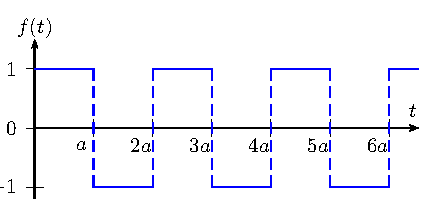
\includegraphics{cap_especiais_coef_var/pics/figura_1}\end{center}
\caption{\label{fig_onda_quadrada}}
\end{figure}
Calculamos a transformada de Laplace usando a propriedade \ref{prop_fun_per} colocando $T=2a$
\begin{eqnarray*}
\mathcal{L}\{f(t)\}&=& \frac{1}{1-e^{-2sa}}\int_0^{2a}f(t)e^{-st}dt\\
&=& \frac{1}{1-e^{-2sa}}\left(\int_0^{a}e^{-st}dt-\int_a^{2a}e^{-st}dt\right)\\
&=& \frac{1}{1-e^{-2sa}}\left(\frac{1-2e^{-as}+e^{-2as}}{s}\right)\\
&=& \frac{1}{(1-e^{-sa})(1+e^{-sa})}\left(\frac{(1-e^{-as})^2}{s}\right)\\
&=&\frac{1}{s} \frac{1-e^{-as}}{1+e^{-sa}}.\\
\end{eqnarray*}
Multiplicando por $e^{\frac{as}{2}}$, podemos escrever a expressão em termos de funções hiperbólicas:
\begin{eqnarray*}
\mathcal{L}\{f(t)\}&=&\frac{1}{s} \frac{e^{\frac{as}{2}}-e^{-\frac{as}{2}}}{e^{\frac{as}{2}}+e^{-\frac{as}{2}})}\\
&=&\frac{1}{s} \frac{\senh\left(\frac{as}{2}\right)}{\cosh\left(\frac{as}{2}\right)}\\
&=&\frac{1}{s} \tanh\left(\frac{as}{2}\right).
\end{eqnarray*}
\end{ex}
\begin{ex}A função $g(t)$ apresentada no gráficoda figura \ref{fig_onda_triangular} é chamada de {\bf onda triangular} de perído $2a$.
 \begin{figure}[!ht]
\begin{center}

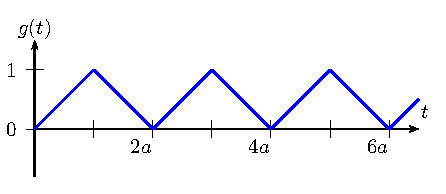
\includegraphics{cap_especiais_coef_var/pics/figura_2}\end{center}
\caption{\label{fig_onda_triangular}}
\end{figure}
Para calcular a transformada de Laplace, observe que:
\begin{itemize}
 \item[a)] A função $g(t)$ representada na figura \ref{fig_onda_triangular} tem como derivada uma onda quadrada. De fato, no intervalo $[0,a]$, a derivada é $\frac{1}{a}$ e no intervalo $[a,2a]$ a derivada é $-\frac{1}{a}$. Esse padrão se repete periodicamente. Logo, a derivada da onda triangular é a onda quadrada multiplicada por $\frac{1}{a}$.
 \item[b)] A propriedade \ref{prop_der} nos dá
 $$
 \mathcal{L}\{g(t)\}=\frac{1}{s}\mathcal{L}\{g'(t)\}+\frac{1}{s}g(0).
 $$
\end{itemize}
Logo,
\begin{eqnarray*}
\mathcal{L}\{\hbox{onda triangular}\}&=&\frac{1}{as}\mathcal{L}\{\hbox{onda quadrada}\}+\frac{1}{s}\hbox{(onda triangular na origem)},
\end{eqnarray*}
e, portanto, usando o fato que a onda triangular vale zero na origem e o resultado do exemplo \ref{ex_onda_quadrada}, temos
\begin{eqnarray*}
\mathcal{L}\{g(t)\}&=&\frac{1}{as}\frac{1}{s} \tanh\left(\frac{as}{2}\right)\\
&=&\frac{1}{as^2} \tanh\left(\frac{as}{2}\right).
\end{eqnarray*}
\end{ex}
\begin{ex} A função $h(t)$ dada por
$$
h(t)=\left\{\begin{array}{ll}\sen(wt),&0<t<\frac{\pi}{w}\\0,& \frac{\pi}{w}<t<\frac{2\pi}{w}, \end{array}\right.,
$$
$h\left(t+\frac{2\pi}{w}\right)=h(t)$, é chamada de {\bf retificador de meia onda} de período $\frac{2\pi}{w}$. A figura \ref{fig_ret_meia_onda} apresenta o gráfico da função $h(t)$.
 \begin{figure}[!ht]
\begin{center}

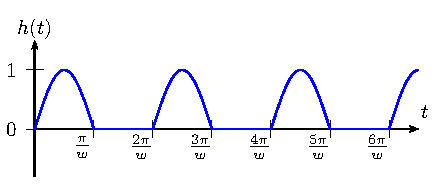
\includegraphics{cap_especiais_coef_var/pics/figura_3}\end{center}
\caption{\label{fig_ret_meia_onda}}
\end{figure}
Calculamos a transformada de Laplace usando a propriedade \ref{prop_fun_per} com $T=\frac{2\pi}{w}$
\begin{eqnarray*}
\mathcal{L}\{f(t)\}&=& \frac{1}{1-e^{-s\frac{2\pi}{w}}}\int_0^{\frac{2\pi}{w}}f(t)e^{-st}dt\\
&=& \frac{1}{1-e^{-s\frac{2\pi}{w}}} \int_0^{\frac{\pi}{w}}\sen(wt)e^{-st}dt\\
&=& \frac{1}{1-e^{-s\frac{2\pi}{w}}} \left[-\frac{e^{-st}\left(\sen(wt)+w\cos(wt)\right)}{s^2+w^2}\right]_0^{\frac{\pi}{w}}\\
&=& \frac{1}{(1-e^{-\frac{s\pi}{w}})(1+e^{-\frac{s\pi}{w}})} \frac{w(1+e^{-\frac{s\pi}{w}})}{s^2+w^2}\\
&=& \frac{1}{1-e^{-\frac{s\pi}{w}}} \frac{w}{s^2+w^2}
\end{eqnarray*}
\end{ex}
\begin{ex} A função $p(t)$ dada por
$$
p(t)=|\sen(wt)|
$$
é chamada de {\bf retificador de onda completa} de período $\frac{\pi}{w}$. A figura \ref{fig_ret_onda_completa} apresenta o gráfico da função $p(t)$.
 \begin{figure}[!ht]
\begin{center}

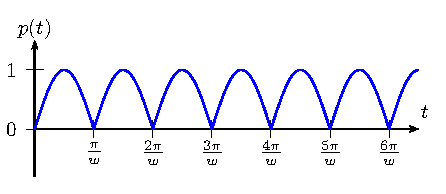
\includegraphics{cap_especiais_coef_var/pics/figura_4}\end{center}
\caption{\label{fig_ret_onda_completa}}
\end{figure}
Calculamos a transformada de Laplace usando a propriedade \ref{prop_fun_per} com $T=\frac{\pi}{w}$
\begin{eqnarray*}
\mathcal{L}\{p(t)\}&=& \frac{1}{1-e^{-s\frac{\pi}{w}}}\int_0^{\frac{\pi}{w}}\sen(wt)e^{-st}dt\\
&=& \frac{1}{1-e^{-s\frac{\pi}{w}}} \left[-\frac{e^{-st}\left(\sen(wt)+w\cos(wt)\right)}{s^2+w^2}\right]_0^{\frac{\pi}{w}}\\
&=& \frac{1}{1-e^{-\frac{s\pi}{w}}} \frac{w(1+e^{-\frac{s\pi}{w}})}{s^2+w^2}\\
&=&  \frac{w}{s^2+w^2}\frac{e^{\frac{s\pi}{2w}}+e^{-\frac{s\pi}{2w}}}{e^{\frac{s\pi}{2w}}-e^{-\frac{s\pi}{2w}}}\\
&=&  \frac{w}{s^2+w^2}\coth\left( \frac{\pi s}{2w}\right)
\end{eqnarray*}
\end{ex}
\begin{ex} A função $q(t)$ dada por
$$
\left\{\begin{array}{ll}q(t)=\frac{t}{a},&0\leq t<a\\ q\left(t+a\right)=q(t), & \end{array}\right.
$$
é chamada de {\bf onda dente de serra} de período $T=a$. A figura \ref{fig_dente_de_serra} apresenta o gráfico da função $q(t)$.
 \begin{figure}[!ht]
\begin{center}

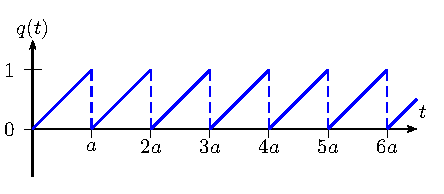
\includegraphics{cap_especiais_coef_var/pics/figura_5}\end{center}
\caption{\label{fig_dente_de_serra}}
\end{figure}
Calculamos a transformada de Laplace usando a propriedade \ref{prop_fun_per} com $T=a$:
\begin{eqnarray*}
\mathcal{L}\{q(t)\}&=& \frac{1}{1-e^{-sa}} \int_0^{a} \frac{t}{a} e^{-st}dt\\
&=&\frac{1}{1-e^{-sa}}\frac{1}{a}\left[ -\frac{e^{-s t} (1+s t)}{s^2}\right]_0^a\\
&=&\frac{1}{1-e^{-sa}}\frac{1-e^{-sa}(1+as)}{s^2a} \\
&=&\frac{1}{1-e^{-sa}}\left(\frac{1-e^{-sa}-e^{-sa} as)}{s^2a} \right)\\
&=&\frac{1}{as^2}-\frac{e^{-sa} }{s\left(1-e^{-sa}\right)}.
\end{eqnarray*}
\end{ex}
\section{Séries de potências}
\subsection{Transformada de Laplace inversa de funções envolvendo expansão em séries de potências}
Em algumas situações, é conveniente expandir em séries de potência um termo de uma função para calcular sua transformada inversa. Vejamos alguns exemplos.
\begin{ex} Vamos calcular a transformada inversa da função $F(s)=\frac{1}{(s+1)(1-e^{-s})}$, usando o fato que
$$\frac{1}{1-e^{-s}}=1+e^{-s}+e^{-2s}+e^{-3s}+\cdots.$$
E, portanto, temos:
 $$ F(s)= \frac{1}{s+1}\left[1+e^{-s}+e^{-2s}+e^{-3s}+\cdots \right]
 $$
 Como, pelo item 7 da tabela de transformadas $\mathcal{L}^{-1}\left\{\frac{1}{s+1}\right\}=e^{-t}.$
Aplicando a propriedade do deslocamento no eixo $t$, temos:
 $$ f(t)= e^{-t}+ u(t-1) e^{-(t-1)}+ u(t-2) e^{-(t-2)}+ u(t-3) e^{-(t-3)}+\cdots.
 $$
O gráfico desta função é apresentado na figura \ref{fig_exp_iterada}.
 \begin{figure}[!ht]
\begin{center}

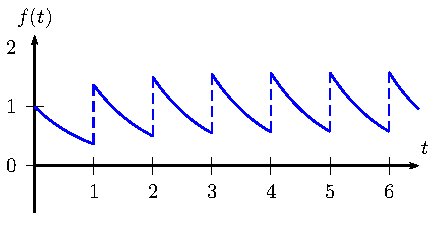
\includegraphics{cap_especiais_coef_var/pics/figura_6}\end{center}
\caption{\label{fig_exp_iterada}}
\end{figure}
\end{ex}
\begin{ex} Vamos calcular a transformada inversa da função $F(s)=\frac{e^{-s}}{s^2}\frac{\left(1-e^{-s}\right)^2}{1-e^{-3s}}$, usando o fato que
$$\frac{1}{1-e^{-3s}}=1+e^{-3s}+e^{-6s}+e^{-9s}+\cdots.$$
Agora observamos que se $g(t)=\mathcal{L}^{-1}\left\{\frac{e^{-s}{\left(1-e^{-s}\right)^2} }{s^2} \right\}$, então:
\begin{eqnarray*}
 g(t)&=&\mathcal{L}^{-1}\left\{\frac{e^{-s}{\left(1-e^{-s}\right)^2} }{s^2} \right\}=\mathcal{L}^{-1}\left\{\frac{e^{-s}\left(1-2e^{-s}+e^{-2s}\right) }{s^2} \right\}\\
 &=&\mathcal{L}^{-1}\left\{\frac{e^{-s}-2e^{-2s}+e^{-3s}}{s^2} \right\} = u(t-1) (t-1) + u(t-2) (4-2t) + u(t-3) (2t-4)
\end{eqnarray*}
Desta forma, pela propriedade do deslocamento em $t$, podemos escrever
\begin{eqnarray*}
f(t)&=&g(t)+u(t-3)g(t-3)+u(t-6)g(t-6)+u(t-9)g(t-9)+\cdots\\
&=&g(t)+g(t-3)+g(t-6)+g(t-9)+\cdots= \sum_{k=0}^\infty g(t-3k)
\end{eqnarray*}
o que implica
$$f(t)= \sum_{k=0}^\infty g(t-3k)=\sum_{k=0}^\infty\left[u(t-1-3k) (t-1-3k) + u(t-2-3k) (4-2t+6k) + u(t-3-3k) (2t-4-6k)\right]$$
O gráfico desta função é apresentado na figura \ref{fig_trian_periodica}.
 \begin{figure}[!ht]
\begin{center}

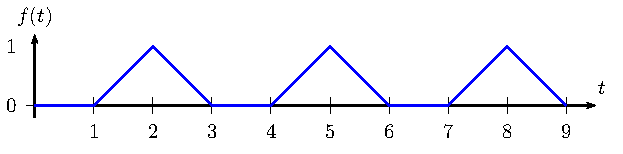
\includegraphics{cap_especiais_coef_var/pics/figura_7}\end{center}
\caption{\label{fig_trian_periodica}}
\end{figure}
\end{ex}
\subsection{Transformada de Laplace de funções envolvendo expansão em séries de potências}
Nesta seção, vamos calcular a transformada de Laplace usando a série de potências das funções e a linearidade da transformada.
\begin{ex}Vamos calcular $\mathcal{L}\{J_0(at)\}$ (item 31 da tabela \ref{tab_trans_Lap_2}), onde $J_0(at)$ é a função de Bessel de ordem zero dada por
$$
J_0(at)=1-\left(\frac{at}{2}\right)^2+\frac{1}{(2!)^2}\left(\frac{at}{2}\right)^4-\frac{1}{(3!)^2}\left(\frac{at}{2}\right)^6+\cdots.
$$
Aplicando o item 3 da tabela \ref{tab_trans_Lap_1}, temos:
\begin{eqnarray*}
\mathcal{L}\left\{J_0(at)\right\}&=&\mathcal{L}\left\{1\right\}-\left(\frac{a}{2}\right)^2\mathcal{L}\left\{t^2\right\}+\frac{1}{(2!)^2}\left(\frac{a}{2}\right)^4\mathcal{L}\left\{t^4\right\}-\frac{1}{(3!)^2}\left(\frac{a}{2}\right)^6\mathcal{L}\left\{t^6\right\}+\cdots\\
&=&\frac{1}{s}-\left(\frac{a}{2}\right)^2\frac{2!}{s^3}+\frac{1}{(2!)^2}\left(\frac{a}{2}\right)^4\frac{4!}{s^5}-\frac{1}{(3!)^2}\left(\frac{a}{2}\right)^6\frac{6!}{s^7}+\cdots\\
&=&\frac{1}{s}\left[1-\frac{1}{2}\left(\frac{a}{s}\right)^2+\frac{1}{2}\cdot \frac{3}{2}\cdot \frac{1}{2!}\left(\frac{a}{s}\right)^4-\frac{1}{2}\cdot\frac{3}{2}\cdot \frac{5}{2}\cdot\frac{1}{3!} \left(\frac{a}{s}\right)^6+\cdots\right]
\end{eqnarray*}
A série acima está apresentada no item 10 da tabela \ref{series_de_potencias}, onde usamos $m=-\frac{1}{2}$ e $x=\left(\frac{a}{s}\right)^2$. Logo,
\begin{eqnarray*}
\mathcal{L}\left\{J_0(at)\right\}&=&\frac{1}{s}\left(1+\left(\frac{a}{s}\right)^2\right)^{-\frac{1}{2}}
\end{eqnarray*}
\end{ex}
\begin{ex}Novamente usamos séries de potências para calcular $\mathcal{L}\{J_0(2\sqrt{kt})\}$, $k>0$ (item 34 da tabela \ref{tab_trans_Lap_2}). Aplicando o item 3 da tabela \ref{tab_trans_Lap_1}, temos:
\begin{eqnarray*}
\mathcal{L}\left\{J_0(2\sqrt{kt})\right\}&=&\mathcal{L}\left\{1-\left(\frac{2\sqrt{kt}}{2}\right)^2+\frac{1}{(2!)^2}\left(\frac{2\sqrt{kt}}{2}\right)^4-\frac{1}{(3!)^2}\left(\frac{2\sqrt{kt}}{2}\right)^6+\cdots\right\}\\
&=&\mathcal{L}\left\{1\right\}-k\mathcal{L}\left\{t\right\}+\frac{k^2}{(2!)^2}\mathcal{L}\left\{t^2\right\}-\frac{k^3}{(3!)^2}\mathcal{L}\left\{t^3\right\}+\cdots\\
&=&\frac{1}{s}-\frac{k}{s^2}+\frac{k^2}{(2!)^2}\frac{2!}{s^3}-\frac{k^3}{(3!)^2}\frac{3!}{s^4}+\cdots\\
&=&\frac{1}{s}\left[1-\left(\frac{k}{s}\right)^1+\frac{1}{2!}\left(\frac{k}{s}\right)^2-\frac{1}{3!}\left(\frac{k}{s}\right)^3+\cdots\right]\\
&=&\frac{1}{s}\left[1+\left(-\frac{k}{s}\right)^1+\frac{1}{2!}\left(-\frac{k}{s}\right)^2+\frac{1}{3!}\left(-\frac{k}{s}\right)^3+\cdots\right]
\end{eqnarray*}
A série acima está apresentada no item 3 da tabela \ref{series_de_potencias}, onde usamos $x=-\frac{k}{s}$. Logo,
\begin{eqnarray*}
\mathcal{L}\left\{J_0(2\sqrt{kt})\right\}&=&\frac{1}{s}e^{-\frac{k}{s}}
\end{eqnarray*}
\end{ex}
\begin{exer}Use o método das séries de potência e as propriedades da função $\Gamma$ para mostrar que
$$
\mathcal{L}\left\{\frac{\cos(2\sqrt{t})}{\sqrt{t}}\right\}=\frac{\sqrt{\pi}}{\sqrt{s}}e^{-\frac{1}{s}}.
$$
\end{exer}
\section{A derivada da transformada de Laplace}
\begin{teo}{\label{prop_der_transf}}(Propriedade da derivada da transformada)
Se $F(s)=\mathcal{L}\{f(t)\}$, então
\begin{equation}
\frac{d}{ds}F(s)=-\mathcal{L}\{tf(t)\}.
\end{equation} 
\end{teo}
\begin{proof}
Usando a definição de transformada de Laplace, temos
\begin{eqnarray*}
\frac{d}{ds}F(s)&=&\frac{d}{ds}\int_0^\infty f(t) e^{-st}dt\\
&=&\int_0^\infty f(t) \frac{d}{ds}\left(e^{-st}\right)dt\\
&=&\int_0^\infty f(t) (-t)e^{-st}dt\\
&=&-\int_0^\infty tf(t) e^{-st}dt\\
&=&-\mathcal{L}\{tf(t)\}.
\end{eqnarray*}
\end{proof}
\begin{ex}Para calcular $\mathcal{L}\{t\cos(wt)\}$, usamos a propriedade \ref{prop_der_transf}:
\begin{eqnarray*}
\mathcal{L}\{t\cos(wt)\}&=&-\frac{d}{ds}\mathcal{L}\{\cos(wt)\}\\
&=&-\frac{d}{ds}\left(\frac{s}{s^2+w^2}\right)\\
&=&-\frac{-s^2+w^2}{(s^2+w^2)^2}\\
&=&\frac{s^2-w^2}{(s^2+w^2)^2}\\
\end{eqnarray*}
\end{ex}
\begin{exer}Calcule $\mathcal{L}\{t^2\sen(wt)\}$ usando a propriedade \ref{prop_der_transf}.
\end{exer}
\section{Equações diferenciais com coeficientes não constantes}
A propriedade \ref{prop_der_transf} da derivada da transformada de Laplace tem uma aplicação importante na solução de equações diferenciais com coeficientes variáveis.
\begin{ex}Vamos resolver o seguinte problema de valor inicial
\begin{eqnarray*}
ty''(t)+y'(t)+9ty(t)&=&0\\
y(0)&=&5\\
y'(0)&=&0.
\end{eqnarray*}
Começamos aplicando a transformada de Laplace na equação diferencial
$$
\mathcal{L}\{ty''(t)\}+\mathcal{L}\{y'(t)\}+9\mathcal{L}\{ty(t)\}=0.
$$
Depois aplicamos a propriedade \ref{prop_der_transf}:
$$
-\frac{d}{ds}\mathcal{L}\{y''(t)\}+\mathcal{L}\{y'(t)\}-9\frac{d}{ds}\mathcal{L}\{y(t)\}=0.
$$
Em seguida aplicamos a propriedade \ref{prop_der} para obter a seguinte equação subsidiária
$$
-\frac{d}{ds}\left(s^2Y(s)-5s\right)+sY(s)-5-9\frac{d}{ds}Y(s)=0,
$$
onde usamos que $y(0)=5$, $y'(0)=0$ e $Y(s)=\mathcal{L}\{y(t)\}$. Agora resolvemos as derivadas e obtemos uma equação diferencial mais simples para $Y(s)$:
$$
-s^2Y'(s)-2sY(s)+sY(s)-9Y'(s)=0,
$$
ou seja,
$$
\frac{Y'(s)}{Y(s)}=-\frac{s}{s^2+9}.
$$
Logo,
$$
\ln(Y(s))=-\frac{1}{2}\ln(s^2+9)+C,
$$
onde $C$ é uma constante de integração. Então
$$
Y(s)=K(s^2+9)^{-\frac{1}{2}}=\frac{K}{\sqrt{s^2+9}},
$$
onde $K=e^{C}$. Pelo item 31 da tabela \ref{tab_trans_Lap_1}, temos
$$
y(t)=KJ_0(3t).
$$
Como $J_0(0)=1$, usamos que $y(0)=5$ para obter $K=5$. Portanto,
$$
y(t)=5J_0(3t).
$$
Observe que a solução satisfaz $y'(0)=0$, porém essa condição não é necessária. De fato, existe uma solução linearmente independente dessa, que não possui transformada de Laplace, pode ser encontrada pelo método das séries de potência.
\end{ex}
\begin{ex}Vamos resolver a equação de Laguerre dada por
$$
ty''(t)+(1-t)y'(t)+2y(t)=0,
$$
com as condições iniciais $y(0)=1$ e $y'(0)=-2$. Primeiro aplicamos a transformada de Laplace nessa equação:
$$
\mathcal{L}\{ty''(t)\}+\mathcal{L}\{y'(t)\}-\mathcal{L}\{ty'(t)\}+2\mathcal{L}\{y(t)\}=0.
$$
Depois usamos a propriedade \ref{prop_der_transf}:
$$
-\frac{d}{ds}\mathcal{L}\{y''(t)\}+\mathcal{L}\{y'(t)\}+\frac{d}{ds}\mathcal{L}\{y'(t)\}+2\mathcal{L}\{y(t)\}=0.
$$
Continuamos usando a propriedade \ref{prop_der} para obter:
$$
-\frac{d}{ds}\left(s^2Y(s)-sy(0)-y'(0)\right)+sY(s)-y(0)+\frac{d}{ds}\left(sY(s)-y(0)\right)+2Y(s)=0,
$$
onde $Y(s)=\mathcal{L}\{y(t)\}$. Aplicando as derivadas chegamos na seguinte equação diferencial para $Y(s)$:
$$
-s^2Y'(s)-2sY(s)+y(0)+sY'(s)+Y(s)+sY(s)-y(0)+2Y(s)=0.
$$
ou seja,
$$
Y'(s)\left(-s^2+s\right)+Y(s)\left(-s+3\right)=0.
$$
Logo,
$$
\frac{Y'(s)}{Y(s)}=-\frac{3-s}{s(1-s)}.
$$
Usamos o método de separação de variáveis para resolver a equação diferencial, temos:
$$
\ln(Y(s))=-\int \frac{3-s}{s(1-s)} ds +C
$$
onde $C$ é uma constante de integração. A antiderivada do lado direito pode ser obtida pelo método de frações parciais:
\begin{eqnarray*}
\frac{-3+s}{s(1-s)}=-\frac{3}{s}-\frac{2}{1-s}.
\end{eqnarray*}
Isso nos dá
$$
\ln(Y(s))=-3\ln(s)+2\ln|1-s|+C=\ln\left(\frac{(1-s)^2}{s^3} \right)+C
$$
ou
$$
Y(s)=K\frac{(1-s)^2}{s^3}=\frac{K}{s^3}-\frac{2K}{s^2}+\frac{K}{s}
$$
onde $K=e^C$. A transformada inversa fornece uma expressão para $y(t)$:
$$
y(t)=K\left(\frac{t^2}{2}-2t+1\right).
$$
Usando o fato que $y(0)=1$, temos $K=1$ e
$$
y(t)=\frac{t^2}{2}-2t+1.
$$
Observe que, apesar da condição para a derivada ser satisfeita, isto é,
$$
y'(0)=0-2=-2,
$$
não usamos-a para calcular a solução. De fato, o problema possui um singularidade na origem que não é percebida pela transformada de Laplace. A solução linearmente independente dessa, que não possui transformada de Laplace, pode ser encontrada pelo método das séries de potência.
\end{ex}
\section{Propriedade da integral da transformada de Laplace}
\begin{teo}{\label{prop_int_transf}}(Propriedade da integral da transformada) Se $F(s)$ é a transformada de Laplace de $f(t)$ e a função
e o limite
$$
\lim_{t\to 0^+}\int_{t}^1\frac{f(\tau)}{\tau}d\tau
$$
existe, então
\begin{equation}
\int_s^\infty F(v)dv =\mathcal{L}\left\{\frac{f(t)}{t}\right\}.
\end{equation}
 \end{teo}
\begin{proof} Usamos a definição de transformada de Laplace para escrever
\begin{eqnarray*}
\int_s^\infty F(v)dv&=&\int_s^\infty\left(\int_0^\infty f(t)e^{-vt}dt\right)dv\\
&=&\int_0^\infty f(t)\left(\int_s^\infty e^{-vt} dv \right)dt\\
&=&\int_0^\infty f(t)\left[\frac{ e^{-vt}}{-t} \right]_s^\infty dt\\
&=&\int_0^\infty \frac{f(t)}{t} e^{-st}  dt\\
&=&\mathcal{L}\left\{ \frac{f(t)}{t} \right\}.
\end{eqnarray*}
Observe que a existência do limite $\lim_{t\to 0^+}\int_{t}^1\frac{f(\tau)}{\tau}d\tau$ é fundamental para a existência da Transformada de Laplace e para os procedimentos analíticos acima.
\end{proof}
\begin{ex}Vamos mostrar o item 29 da tabela \ref{tab_trans_Lap_2}:
$$
\mathcal{L}\left\{\frac{1}{2\sqrt{\pi t^3}}\left(e^{bt}-e^{at}\right)\right\}=\sqrt{s-a}-\sqrt{s-b}.
$$
Para isso vamos usar o item 4, a saber,
\begin{equation}{\label{eq_item_4}}
\mathcal{L}\left\{\frac{1}{\sqrt{\pi t}}\right\}=\frac{1}{\sqrt{s}}.
\end{equation}
Aplicamos a propriedade \ref{prop_trans_s} da translação no eixo $s$ na equação (\ref{eq_item_4}) para obter:
\begin{equation*}
\mathcal{L}\left\{\frac{1}{\sqrt{\pi t}}e^{at}\right\}=\frac{1}{\sqrt{s-a}}.
\end{equation*}
Finalmente, usando a propriedade \ref{prop_int_transf} da integral da transformada, obtemos:
\begin{eqnarray*}
\mathcal{L}\left\{\frac{1}{2\sqrt{\pi t^3}}\left(e^{bt}-e^{at}\right)\right\}&=&\frac{1}{2}\mathcal{L}\left\{\frac{1}{t}\left(\frac{1}{\sqrt{\pi t}}e^{bt}-\frac{1}{\sqrt{\pi t}}e^{at}\right)\right\}\\
&=&\frac{1}{2}\int_s^\infty\left(   \frac{1}{\sqrt{v-b}}-  \frac{1}{\sqrt{v-a}}\right)dv\\
&=&\frac{1}{2}\int_s^\infty  \left( \left(v-b\right)^{-\frac{1}{2}}-  \left(v-a\right)^{-\frac{1}{2}}\right)dv\\
&=&\left. -\left(v-b\right)^{\frac{1}{2}}+ \left(v-a\right)^{\frac{1}{2}}\right|_s^\infty\\
&=&\sqrt{s-a}-\sqrt{s-b}.
\end{eqnarray*}
Observe que aqui usamos o seguinte limite no infinito
\begin{eqnarray*}
\lim_{v\to\infty}\left( \sqrt{v-b}- \sqrt{v-a}\right)&=&\lim_{v\to\infty}\frac{\left(\sqrt{v-b}- \sqrt{v-a}\right)\left(\sqrt{v-b}+ \sqrt{v-a}\right)}{\left(\sqrt{v-b}+ \sqrt{v-a}\right)}\\
&=&\lim_{v\to\infty}\frac{\left((v-b)- (v-a)\right)}{\left(\sqrt{v-b}+ \sqrt{v-a}\right)}\\
&=&\lim_{v\to\infty}\frac{\left(a-b\right)}{\left(\sqrt{v-b}+ \sqrt{v-a}\right)}\\
&=&0.
\end{eqnarray*}
\end{ex}
\begin{ex}Vamos mostrar o item 39 da tabela \ref{tab_trans_Lap_2}:
$$
\mathcal{L}\left\{\frac{1}{t}\left(e^{bt}-e^{at}\right)\right\}=\ln\left(\frac{s-a}{s-b}\right).
$$
Para isso vamos usar o item 7, a saber,
\begin{equation*}
\mathcal{L}\left\{e^{at}\right\}=\frac{1}{s-a}.
\end{equation*}
Usando a propriedade \ref{prop_int_transf} da integral da transformada, obtemos:
\begin{eqnarray*}
\mathcal{L}\left\{\frac{1}{t}\left(e^{bt}-e^{at}\right)\right\}&=&\int_s^\infty \left(\frac{1}{v-b}-\frac{1}{v-a}\right)dv\\
&=& \left.\left(\ln(v-b)-\ln(v-a)\right)\right|_s^\infty\\
&=& \left(\ln(s-a)-\ln(s-b)\right)\\
&=&\ln\left(\frac{s-a}{s-b}\right)
\end{eqnarray*}
Na penúltima igualdade usamos o seguinte limite no infinito:
\begin{eqnarray*}
\lim_{v\to\infty} \left(\ln(v-b)-\ln(v-a)\right)&=&\lim_{v\to\infty} \ln\left(\frac{v-b}{v-a}\right)\\
&=& \ln\left(\lim_{v\to\infty}\left(\frac{v-b}{v-a}\right)\right)\\
&=& \ln\left(1\right)\\
&=&0.
\end{eqnarray*}
Observe que a troca do limite com o logarítmo é possível visto que $\ln(x)$ é contínua para $x>0$.
\end{ex}
\begin{ex}Vamos mostrar o item 40 da tabela \ref{tab_trans_Lap_2}:
$$
\mathcal{L}\left\{\frac{2}{t}\left(1-\cos(wt)\right)\right\}=\ln\left(\frac{s^2+w^2}{s^2}\right).
$$
Para isso vamos usamos o fato que
\begin{equation*}
\mathcal{L}\left(1-\cos(wt)\right)=\frac{1}{s}-\frac{s}{s^2+w^2}.
\end{equation*}
Usando a propriedade \ref{prop_int_transf} da integral da transformada, obtemos:
\begin{eqnarray*}
\mathcal{L}\left\{\frac{2}{t}\left(1-\cos(wt)\right)\right\}&=&2\int_s^\infty \left(\frac{1}{v}-\frac{v}{v^2+w^2}\right)dv\\
&=& \left.2\left(\ln(v)-\frac{1}{2}\ln(v^2+w^2)\right)\right|_s^\infty\\
&=& \left.\left(2\ln(v)-\ln(v^2+w^2)\right)\right|_s^\infty\\
&=&\left.\ln\left(\frac{v^2}{v^2+w^2}\right)\right|_s^\infty\\
&=&-\ln\left(\frac{s^2}{s^2+w^2}\right)\\
&=&\ln\left(\frac{s^2+w^2}{s^2}\right)
\end{eqnarray*}
Na penúltima igualdade usamos o seguinte limite no infinito:
\begin{eqnarray*}
\lim_{v\to\infty} \ln\left(\frac{v^2}{v^2+w^2}\right)&=& \ln\left(\lim_{v\to\infty}\left(\frac{v^2}{v^2+w^2}\right)\right)\\
&=& \ln\left(1\right)\\
&=&0.
\end{eqnarray*}
Observe que a troca do limite com o logarítmo é possível visto que $\ln(x)$ é contínua para $x>0$.
\end{ex}
\begin{exer}Demonstre o item 41 da tabela usando os itens 1 e 16 juntamente com a propriedade \ref{prop_int_transf}.
\end{exer}
\begin{ex}{\label{ex_sint_t}}Vamos demonstrar o item 42 da tabela \ref{tab_trans_Lap_2}:
$$
\mathcal{L}\left\{\frac{1}{t}\sen(wt)\right\}=\arctan\left(\frac{w}{s}\right).
$$
Para isso vamos usamos o fato que
\begin{equation*}
\mathcal{L}\{\sen(wt)\}=\frac{w}{s^2+w^2}.
\end{equation*}
Usando a propriedade \ref{prop_int_transf} da integral da transformada, obtemos:
\begin{eqnarray*}
\mathcal{L}\left\{\frac{1}{t}\sen(wt)\right\}&=&\int_s^\infty \left(\frac{w}{v^2+w^2}\right)dv\\
&=& \left.\arctan\left(\frac{v}{w}\right)\right|_s^\infty\\
&=&\lim_{v\to\infty}\arctan\left(\frac{v}{w}\right)-\arctan\left(\frac{s}{w}\right)\\
&=&\frac{\pi}{2}-\arctan\left(\frac{s}{w}\right)\\
\end{eqnarray*}
Usando o fato que $\tan\left(\frac{\pi}{2}-\theta\right)=\cot(\theta)$, temos que
\begin{eqnarray*}
\mathcal{L}\left\{\frac{1}{t}\sen(wt)\right\}=\cot^{-1}\left(\frac{s}{w}\right).
\end{eqnarray*}
Também, se $\gamma=\cot^{-1}\left(\frac{s}{w}\right)$, então $\cot\gamma=\frac{s}{w}$. Logo, $\frac{1}{\tan\gamma}=\frac{s}{w}$ e, portanto, $\tan\gamma=\frac{w}{s}$. Assim, podemos escrever a transformada de Laplace da seguinte forma:
\begin{eqnarray*}
\mathcal{L}\left\{\frac{1}{t}\sen(wt)\right\}=\arctan\left(\frac{w}{s}\right)
\end{eqnarray*}
\end{ex}
\begin{ex}Vamos agora mostrar o item 43 da tabela \ref{tab_trans_Lap_2}:
$$
\mathcal{L}\left\{\hbox{Si}\ \!(t)\right\}=\frac{1}{s}\cot^{-1}(s),
$$
onde $\hbox{Si}\ \!(t)$ é função integral seno dada por:
$$
\hbox{Si}\ \!(t)=\int_0^t\frac{\sen(x)}{x}dx.
$$
Primeiro aplicamos a propriedade \ref{prop_trans_int} para obter
$$
\mathcal{L}\left\{\hbox{Si}\ \!(t)\right\}=\mathcal{L}\left\{\int_0^t\frac{\sen(x)}{x}dx\right\}=\frac{1}{s}\mathcal{L}\left\{\frac{\sen(t)}{t}\right\}.
$$
Em seguida usamos o resultado do exemplo \ref{ex_sint_t} (ou item 42 da tabela \ref{tab_trans_Lap_2}) e temos:
$$
\mathcal{L}\left\{\hbox{Si}\ \!(t)\right\}=\frac{1}{s}\arctan\left(\frac{1}{s}\right)=\frac{1}{s}\cot^{-1}\left(s\right).
$$
\end{ex}
\section{Propriedades do Valor Inicial e Final}
\begin{teo}(Propriedade do Valor Final) Se $F(s)$ é a transformada de Laplace de $f(t)$ e 
$$
\lim_{t\to\infty}f(t)=L,
$$
então
$$
\lim_{s\to 0^+} sF(s)=L.
$$
\end{teo}
\begin{proof}Usamos a definição de transformada de Laplace para escrever
\begin{eqnarray*}
sF(s)&=&s\int_0^\infty f(t)e^{-st}dt\\
&=&s\int_0^a f(t)e^{-st}dt+s\int_a^\infty f(t)e^{-st}dt.\\
\end{eqnarray*}
Observe que a primeira parcela do lado direito tende a zero independentemente do valor de $a$. Porém, para $a$ suficientemente grande, $f(t)$ se aproxima de $L$, pois $\displaystyle \lim_{t\to\infty}f(t)=L$, ou seja,
\begin{eqnarray*}
s\int_a^\infty f(t)e^{-st}dt &\approx &s\int_a^\infty L e^{-st}dt.\\
&\approx &s\frac{L}{-s}\left[ e^{-st}\right]_a^\infty=Le^{-as}
\end{eqnarray*}
Como $e^{-as}\to 1$ quando $s\to 0$, então
$$
\lim_{s\to 0^+} sF(s)=L.
$$ 
\end{proof}
\begin{teo}(Propriedade do Valor Inicial) Se $F(s)$ é a transformada de Laplace de uma função $f(t)$ de ordem exponencial $c$ e 
$$
\lim_{t\to 0^+}f(t)=L,
$$
então
$$
\lim_{s\to \infty} sF(s)=L.
$$
\end{teo}
\begin{proof}Usamos a definição de transformada de Laplace para escrever
\begin{eqnarray*}
sF(s)&=&s\int_0^\infty f(t)e^{-st}dt\\
&=&s\int_0^a f(t)e^{-st}dt+s\int_a^b f(t)e^{-st}dt+s\int_b^\infty f(t)e^{-st}dt.\\
\end{eqnarray*}
Observe que a segunda parcela do lado direito tende a zero quando $s\to \infty$ independentemente do valor de $a$ e $b$, pois o fato da função ser de ordem exponencial e contínua por partes implica em $f(t)$ limitada em $[a,b]$, ou seja, $|f(t)|<M$ e, portanto,
\begin{eqnarray*}
\left|s\int_a^b f(t)e^{-st}dt\right|&\leq & s\int_a^b |f(t)|e^{-st}dt\\
&\leq & Ms\int_a^b e^{-st}dt\\
&\leq & \left.Ms\frac{1}{-s} e^{-st}\right|_a^b=M(e^{-sa}-e^{-sb}).
\end{eqnarray*}
Também, a terceira parcela tende a zero se $b$ for suficientemente grande, pois existem $c$ e $M>0$ tal que $|f(t)|<Me^{ct}$ para $t>b$ e, portanto,
\begin{eqnarray*}
\left|s\int_b^\infty f(t)e^{-st}dt\right|&\leq & s\int_b^\infty |f(t)|e^{-st}dt\\
&\leq & s\int_b^\infty Me^{-(s-c)t}dt\\
&\leq & \left.Ms\frac{1}{c-s} e^{-(s-c)t}\right|_b^\infty=\frac{Ms}{s-c}(e^{-(s-c)b}).
\end{eqnarray*}
Porém, para $a$ suficientemente pequeno, $f(t)$ se aproxima de $L$, pois $\displaystyle \lim_{t\to 0}f(t)=L$, ou seja,
\begin{eqnarray*}
s\int_0^a f(t)e^{-st}dt &\approx &s\int_0^a L e^{-st}dt.\\
&\approx &s\frac{L}{-s}\left[ e^{-st}\right]_0^a=L\left(1-e^{-as}\right)
\end{eqnarray*}
Como $e^{-as}\to 0$ quando $s\to \infty$, então
$$
\lim_{s\to \infty} sF(s)=L.
$$ 
\end{proof}
\section{Exercícios}
\begin{Exercise}
 Demonstre o item (32) da tabela usando os itens (4) e (5) e a propriedade \ref{prop_trans_s} do deslocamento no eixo $s$. 
\end{Exercise}
\begin{Exercise}
Use a propriedade da derivada da transformada para calcular $\displaystyle \mathcal{L}\{ t \cos (\omega t) \}$. A partir desta, prove que $$ \mathcal{L}\{ \sen (\omega t) - \omega t \cos (\omega t) \} = \frac{2 \omega^3 }{(s^2 + \omega^2)^2}. $$
\end{Exercise}
\begin{Exercise}
Encontre a transformada inversa das funções abaixo utlizando o método que achar adequado.
\begin{itemize}
\item[a)] $\displaystyle F(s)= \frac{3s + 7}{s^2 - 2 s - 3}$.
\item[b)] $\displaystyle F(s)= \frac{1}{(s-2)^3}$.
\item[c)] $\displaystyle F(s)= \frac{3s + 1}{(s-1)(s^2 +1)}$.
\item[d)] $\displaystyle F(s)= \frac{s + 12}{s^2 +4s}$.
\item[e)] $\displaystyle F(s)= \frac{s -3}{s^2 -1}$.
\item[f)] $\displaystyle F(s)= \frac{3s}{s^2 +2s -8}$.
\item[g)] $\displaystyle F(s)= \frac{3s^2 -2s - 1}{(s-3)(s^2 +1)}$.
\item[h)] $\displaystyle F(s)= \frac{s + 1}{s^2 +4s +13}$.
\item[i)] $\displaystyle F(s)= \frac{s^2 + s -2}{(s +1)^3}$.
\item[j)] $\displaystyle F(s)= \frac{2s^3 +10s^2+8s+40}{s^2(s^2 +9)}$.
\item[k)] $\displaystyle F(s)= \frac{2s^2 -4}{(s+1)(s-2)(s-3)}$.
\item[l)] $\displaystyle F(s)= \frac{1}{(s^2+4)(s^2 +1)}$.
\end{itemize}
\end{Exercise}
\begin{resp}
\begin{itemize}
  \item[a)] $\displaystyle f(t) = 4e^{3t} - e^{-t}$
  \item[b)] $\displaystyle f(t) = \frac{1}{2} t^2 e^{2t}$
  \item[c)] $\displaystyle f(t) = 2e^{t} - 2 \cos t + \sen t$
  \item[d)] $\displaystyle f(t) = 3 -2 e^{-4t}$
  \item[e)] $\displaystyle f(t) = \cosh t - 3 \senh t$
  \item[f)] $\displaystyle f(t) = 2e^{-4t} + e^{2t}$
  \item[g)] $\displaystyle f(t) = 2e^{3t} + \cos t + \sen t$
  \item[h)] $\displaystyle f(t) = e^{-2t}\bigg[ \cos(3t) - \frac{1}{3} \sen (3t) \bigg]$
  \item[i)] $\displaystyle f(t) = e^{-t}(1-t-t^2)$
  \item[j)] $\displaystyle f(t) = 2\cos(3t) +\frac{10}{3} \sen(3t) +\frac{8}{9} \big[1-\cos(3t)\big] + \frac{40}{27} \big[3t - \sen(3t)\big]$
  \item[k)] $\displaystyle f(t) = -\frac{1}{6} e^{-t} -\frac{4}{3} e^{2t} + \frac{7}{2} e^{3t}$
  \item[l)] $\displaystyle f(t) = \frac{1}{3} \bigg[ \sen t - \frac{1}{2}\sen(2t) \bigg]$
\end{itemize}
\end{resp}
\begin{Exercise}
Use a tabela da transformada de Laplace para mostrar que:
\begin{itemize}
  \item[a)] $\displaystyle \mathcal{L} \big\{ t^{1/2}+ t^{-1/2} \big\} = \frac{\sqrt{\pi}(2s+1)}{2s^{3/2}}$
  \item[b)] $\displaystyle \mathcal{L} \bigg\{ \frac{e^{-2t}}{\sqrt{t}} \bigg\} = \sqrt{\frac{\pi}{s+2}}$
  \item[c)] $\displaystyle \mathcal{L} \bigg\{ \frac{\cos(2\sqrt{t}) }{\sqrt{t}} \bigg\} = e^{-1/s}\sqrt{\frac{\pi}{s}}$
\end{itemize}
\end{Exercise}
\begin{Exercise}
Use o método das séries de potências para mostrar que \[\mathcal{L} \{\sen \sqrt{t} \} =  \frac{\sqrt{\pi} e^{-1/4s}}{2s^{3/2}}.\]
\emph{Sugestão}: Use que \[\Gamma\bigg( n + \frac{3}{2} \bigg) = \frac{ (2n+1)!}{ n! 2^{2n+1}}\sqrt{\pi}.\]
\end{Exercise}
\begin{resp}
 \begin{eqnarray*}
f(t)&=&\sin\sqrt{t}= \sum_{n=0}^{\infty}(-1)^n\frac{t^{(2n+1)/2}}{(2n+1)!}\\
F(s)&=&\mathcal{L}\left\{f(t)\right\}=\sum_{n=0}^{\infty}\frac{(-1)^n}{{(2n+1)!}}\mathcal{L}\left\{{t^{(2n+1)/2}}\right\}\\
&=&\sum_{n=0}^{\infty}\frac{(-1)^n}{{(2n+1)!}}\mathcal{L}\left\{{t^{(2n+1)/2}}\right\}\\
&=&\sum_{n=0}^{\infty}\frac{(-1)^n}{{(2n+1)!}}\Gamma\left((2n+3)/2\right)\frac{1}{s^{(2n+3)/2}}\\
&=&\sum_{n=0}^{\infty}\frac{(-1)^n}{{(2n+1)!}}\frac{(2n+1)!}{n!}\frac{\sqrt{\pi}}{2^{2n+1}}\frac{1}{s^{(2n+3)/2}}\\
&=&\frac{\sqrt{\pi}}{2s^{3/2}}\sum_{n=0}^{\infty}{(-1)^n}\frac{1}{n!}\frac{1}{2^{2n}}\frac{1}{s^{n}}\\
&=&\frac{\sqrt{\pi}}{2s^{3/2}}\sum_{n=0}^{\infty}\frac{1}{n!}{\left(-\frac{1}{4s}\right)^{n}}\\
&=&\frac{\sqrt{\pi}}{2s^{3/2}}e^{-\frac{1}{4s}}
\end{eqnarray*}
Para mostrar a identidade $\Gamma\bigg( n + \frac{3}{2} \bigg) = \frac{ (2n+1)!}{ n! 2^{2n+1}}\sqrt{\pi}$ , usamos a relação de recorrência
$$\Gamma(x+1)=x\Gamma(x)$$
e o fato bem conhecido  de que
$$\Gamma(1/2)=\sqrt{\pi}$$
Para obter
\begin{eqnarray*}
\Gamma(3/2)&=&\Gamma(1+1/2)=\frac{1}{2}\Gamma(1/2)=\frac{\sqrt{\pi}}{2}\\
\Gamma(5/2)&=&\Gamma(1+3/2)=\frac{3}{2}\Gamma(3/2)=\frac{3\sqrt{\pi}}{2^2}\\
\Gamma(7/2)&=&\Gamma(1+5/2)=\frac{5}{2}\Gamma(5/2)=\frac{5 \cdot 3\sqrt{\pi}}{2^3}\\
\Gamma(9/2)&=&\Gamma(1+7/2)=\frac{7}{2}\Gamma(7/2)=\frac{7\cdot 5 \cdot 3\sqrt{\pi}}{2^4}\\
\end{eqnarray*}
E generalizando, temos:
\begin{eqnarray*}
\Gamma\left(\frac{2n+1}{2}\right)&=&\Gamma\left(1+\frac{2n-1}{2}\right)=\frac{2n-1}{2}\Gamma\left(\frac{2n-1}{2}\right)={(2n-1)(2n-3)\cdots 3}\frac{\sqrt{\pi}}{2^{n}}\\
&=&\frac{(2n-1)(2n-2)(2n-3)\cdots 3\cdot 2 \cdot 1}{(2n-2)(2n-4)\cdots 2}\frac{\sqrt{\pi}}{2^{n}}\\
&=&\frac{(2n-1)(2n-2)(2n-3)\cdots 3\cdot 2 \cdot 1}{2^{n-1}(n-1)(n-2)\cdots 1}\frac{\sqrt{\pi}}{2^{n}}\\
&=&\frac{(2n-1)!}{(n-1)!}\frac{\sqrt{\pi}}{2^{2n-1}}
\end{eqnarray*}
\end{resp}
\begin{Exercise}
Usando a derivada da transformada de Laplace, calcule:
\begin{itemize}
  \item[a)] $\displaystyle \mathcal{L} \{ t \senh (at) \}$
  \item[b)] $\displaystyle \mathcal{L} \{ t \cosh (at) \}$
\end{itemize}
\end{Exercise}
\begin{resp}
 \begin{itemize}
  \item[a)] $\displaystyle \frac{2as}{(s^2 - a^2)^2}$
  \item[b)] $\displaystyle \frac{s^2 + 9}{(s^2 - 9)^2}$
 \end{itemize}
\end{resp}
\begin{Exercise}
Resolva
\[
\left\{
  \begin{array}{ll}
    ty'' (t) + 2y'(t) +ty(t) = 0 \\
    y(0)=1, \quad y(\pi) = 0
  \end{array}
\right.
\] \emph{Sugestão}: Utilize que $\displaystyle \lim_{s\to + \infty} Y(s) = 0.$
\end{Exercise}
\begin{resp}
 $\displaystyle y(t) = \frac{\sen t}{t}$
\end{resp}
\begin{Exercise}
Utilize a integral da transformada de Laplace para demonstrar que:
\begin{itemize}
  \item[a)] $\displaystyle \mathcal{L}\bigg\{ \frac{\senh t}{t} \bigg\} = \frac{1}{2} \ln \bigg(\frac{s+1}{s-1}\bigg)$
  \item[b)] $\displaystyle \mathcal{L}\bigg\{ \frac{2}{t} \big( 1 - \cos (\omega t) \big) \bigg\} = \ln \bigg(\frac{s^2 + \omega^2}{s^2}\bigg)$
  \item[c)] $\displaystyle \mathcal{L}\bigg\{ \frac{2}{t} \big( 1 - \cosh (\omega t) \big) \bigg\} = \ln \bigg(\frac{s^2 - \omega^2}{s^2}\bigg)$
\end{itemize}
\end{Exercise}
\begin{resp}
 \begin{itemize}
  \item[a)] $\displaystyle \frac{ 3 - 3 e^{-2s} - 6s e^{-4s} }{s^2 (1 - e^{-4s})}$
  \item[b)] $\displaystyle \frac{  e^{2\pi(1-s)} -1 }{(1-s) (1 - e^{-2\pi s})}$
  \item[c)] $\displaystyle \frac{\omega}{s^2 + \omega^2} \coth \bigg(\frac{\pi s}{2 \omega^2} \bigg)$
 \end{itemize}
\end{resp}
\begin{Exercise}
Faça o gráfico de $f(t)$ e calcule $\mathcal{L}\big\{f(t)\big\}$.
\begin{itemize}
  \item[a)] $f$ periódica de período $p=4$ e $\displaystyle f(t) = \left\{
                                                                      \begin{array}{ll}
                                                                        3t, & \hbox{ se } t \in (0,2) \\
                                                                        6, & \hbox{ se } t \in (2,4)
                                                                      \end{array}
                                                                    \right.
$
  \item[b)] $f$ periódica de período $p=2\pi$ e $\displaystyle f(t) = e^t$, para $t \in (0,2\pi)$.
  \item[b)] $\displaystyle f(t) = |\sen (\omega t)|$.
\end{itemize}
\end{Exercise}
\begin{resp}
 \begin{itemize}
  \item[a)] $\displaystyle y(t) = 10 \cos (2t) + \frac{k}{8} \Big( 1 - \cos \big(2(t-a)\big) \Big)u(t-a) $
  \item[b)] $\displaystyle y(t) = 10 \cos (2t) + \frac{k}{4} \sen(2t)$
 \end{itemize}
\end{resp}
\begin{Exercise}
Para $k$ constante, encontre a solução de
\begin{itemize}
  \item[a)] $\displaystyle \left\{
                              \begin{array}{ll}
                                2y''(t) + 8 y(t) = k u(t-a) \\
                                y(0)=10, y'(0)=0
                              \end{array}
                            \right.
$
  \item[b)] $\displaystyle \left\{
                              \begin{array}{ll}
                                2y''(t) + 8 y(t) = k \delta(t) \\
                                y(0)=10, y'(0)=0
                              \end{array}
                            \right.
$
\end{itemize}
\end{Exercise}
\begin{Exercise}
Considere o OHS não amortecido representado na figura \ref{massa-mola-1}. Suponha que, em $t=0$, a massa $m$ está em sua posição de equilíbrio. Encontre o deslocamento $x(t)$ para $t>0$, se uma força $F_0 \delta(t)$ é aplicada.
\begin{figure}[!ht]
\begin{center}

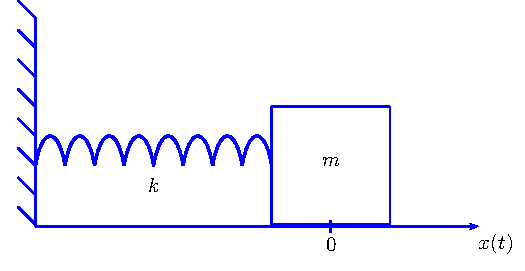
\includegraphics{cap_especiais_coef_var/pics/figura_8}\end{center}
\caption{\label{massa-mola-1}}
\end{figure} 
\end{Exercise}
\begin{resp}
  $\displaystyle y(t) = \frac{F_0}{\sqrt{km}} \sen \left(\sqrt{\frac{k}{m}} t\right)$
\end{resp}
